\documentclass{article}

% if you need to pass options to natbib, use, e.g.:
% \PassOptionsToPackage{numbers, compress}{natbib}
% before loading nips_2016
%
% to avoid loading the natbib package, add option nonatbib:
% \usepackage[nonatbib]{nips_2016}

\usepackage{nips_2016}

% to compile a camera-ready version, add the [final] option, e.g.:
% \usepackage[final]{nips_2016}

\usepackage[utf8]{inputenc} % allow utf-8 input
\usepackage[T1]{fontenc}    % use 8-bit T1 fonts
%\usepackage{hyperref}       % hyperlinks
\usepackage{url}            % simple URL typesetting
\usepackage{booktabs}       % professional-quality tables
\usepackage{amsfonts}       % blackboard math symbols
\usepackage{nicefrac}       % compact symbols for 1/2, etc.
\usepackage{microtype}      % microtypography
\usepackage{amsmath}
\usepackage{mathtools}
\usepackage{fancyvrb}
\usepackage{multirow}
\usepackage{color}

\usepackage{listings}
\definecolor{lightgray}{rgb}{.9,.9,.9}
\definecolor{darkgray}{rgb}{.4,.4,.4}
\definecolor{purple}{rgb}{0.65, 0.12, 0.82}
\definecolor{orange}{rgb}{1,0.5,0}

\definecolor{Red}{RGB}{255,0,0}
\newcommand{\red}[1]{\textcolor{Red}{#1}}
\definecolor{Green}{RGB}{10,200,100}
\definecolor{Blue}{RGB}{10,100,200}
\newcommand{\ndg}[1]{\textcolor{Green}{[ndg: #1]}}
\newcommand{\mht}[1]{\textcolor{Blue}{[mht: #1]}}
\newcommand{\lou}[1]{\textcolor{orange}{[lou: #1]}}

\lstdefinelanguage{JavaScript}{
  keywords={typeof, new, true, false, catch, function, return, null, catch, switch, var, if, in, while, do, else, case, break},
  keywordstyle=\color{blue}\bfseries,
  ndkeywords={class, export, boolean, throw, implements, import, this},
  ndkeywordstyle=\color{darkgray}\bfseries,
  identifierstyle=\color{black},
  sensitive=false,
  comment=[l]{//},
  morecomment=[s]{/*}{*/},
  commentstyle=\color{purple}\ttfamily,
  stringstyle=\color{red}\ttfamily,
  morestring=[b]',
  morestring=[b]"
}

\lstset{
   language=JavaScript,
   backgroundcolor=\color{white},
   extendedchars=true,
   basicstyle=\footnotesize\ttfamily,
   showstringspaces=false,
   showspaces=false,
   numbers=none,
   numberstyle=\footnotesize,
   numbersep=9pt,
   tabsize=2,
   breaklines=true,
   showtabs=false,
   captionpos=b
}



\usepackage[ruled,vlined]{algorithm2e}

\newcommand{\ud}{\,\mathrm{d}}
\newcommand{\argmax}{\operatornamewithlimits{argmax}}


\title{Practical optimal experiment design for psychology}

% The \author macro works with any number of authors. There are two
% commands used to separate the names and addresses of multiple
% authors: \And and \AND.
%
% Using \And between authors leaves it to LaTeX to determine where to
% break the lines. Using \AND forces a line break at that point. So,
% if LaTeX puts 3 of 4 authors names on the first line, and the last
% on the second line, try using \AND instead of \And before the third
% author name.

\author{
  David S.~Hippocampus\thanks{Use footnote for providing further
    information about author (webpage, alternative
    address)---\emph{not} for acknowledging funding agencies.} \\
  Department of Computer Science\\
  Cranberry-Lemon University\\
  Pittsburgh, PA 15213 \\
  \texttt{hippo@cs.cranberry-lemon.edu} \\
  %% examples of more authors
  %% \And
  %% Coauthor \\
  %% Affiliation \\
  %% Address \\
  %% \texttt{email} \\
  %% \AND
  %% Coauthor \\
  %% Affiliation \\
  %% Address \\
  %% \texttt{email} \\
  %% \And
  %% Coauthor \\
  %% Affiliation \\
  %% Address \\
  %% \texttt{email} \\
  %% \And
  %% Coauthor \\
  %% Affiliation \\
  %% Address \\
  %% \texttt{email} \\
}

\begin{document}
% \nipsfinalcopy is no longer used

\maketitle

\begin{abstract}
  The abstract paragraph should be indented \nicefrac{1}{2}~inch
  (3~picas) on both the left- and right-hand margins. Use 10~point
  type, with a vertical spacing (leading) of 11~points.  The word
  \textbf{Abstract} must be centered, bold, and in point size 12. Two
  line spaces precede the abstract. The abstract must be limited to
  one paragraph.
\end{abstract}

\section{Introduction}
\ndg{Doing the standard, active learning thing with probabilistic programs. }

Designing scientific experiments is hard.
At the very least, you must have a hypothesis in hand, a space of possible experiments, and clarity to reason through the logic of your hypothesis in each possible experiment.
Experiments on human behavior have a number of added complications.
For instance, human data is noisy and sensitive to dependent measure of the task. Further, human data costs money and deciding on the number of participants for a study is another crucial decision variable.

Formal models of psychological phenomena are used to make specific hypotheses about observed data.
These hypotheses are more explicit than what can be achieved using verbal or qualitative theories. Despite the rising popularity of formal models in psychology, experiment design is still largely confined to the realm of expert intuition and folk theory.
We present a general, turn-key approach to designing experiments that best disambiguates competing hypotheses using a Bayesian framework.
Though the framework is Bayesian, it is not directly related to Bayesian models of cognition; rather, it can be applied to any instance in which the scientist has a formal model of the data generating process (including, Bayesian models of cognition).

We are not the first to attempt to develop a framework for optimal experiments in psychology. Previous attempts, however, suffer from a number of pragmatic issues that impede the psychologist who wishes to readily apply optimal experiment design (OED) to their research.
These include ad-hoc optimization criteria, which put the burden on researchers to have sufficient expertise to select a criterion;
a lack of established pipeline, requiring researchers to develop their own system for writing formal psychological models and the OED optimization engine;
and a lack of analysis in dealing with practical experimental concerns in psychology, including dealing with noisy responses from participants, determining ideal numbers of participants, and deciding upon appropriate dependent measures or linking functions.

In this paper, we introduce practical optimal experiment design for psychological research using a Bayesian model selection framework.
We apply this framework to two case studies: subjective randomness and categorization.
The first case study highlights the details of application for a simple space of experiments.
The second study applies OED to a larger space of possible experiments and validates our theoretical analysis by running the optimal experiment.
We conclude by highlighting the generality of the approach and areas of future work.


\ndg{all the parts are here. needs smoothing. make it clearer that using PPL to represent hypotheses is a key step in making the system practical.}

%    \begin{itemize}
%        \item It is difficult to discriminate models of psychological processes
%        \item Experiments are expensive
%        \item We present a general, turn-key approach to design experiments that best disambiguate competing models using a Bayesian framework
%        \item This technique is not directly related to Bayesian models of cognition. It can be used on any (formal / probabilistic) model, including Bayesian models of cognition
%        \item Despite the previous attempts in this field, there are a number of pragmatic issues that make it difficult to readily apply OED techniques for psychology, including:
%        \begin{itemize}
%            \item A variety of proposed optimization criteria, which puts the burden on researchers to have sufficient expertise to select the appropriate approach
%            \item A lack of an established pipeline, requiring researchers to develop a language to formalize psychological models and write an OED optimization engine
%            \item A lack of analysis in dealing with practical experimental concerns such as:
%                \begin{itemize}
%                    \item Noisy responses from participants
%                    \item The ideal number of participants for a study
%                    \item The ambiguity of linking functions of dependent measures
%                \end{itemize}
%        \end{itemize}
%    \end{itemize}


\section{Bayesian model selection framework}
\label{s:bayes}

\ndg{add a high-level overview of the setup first. describe the most general formulation (cognitive model of responses) and the more parsimonious bayesian modeling version where the response distribution is factored into belief-update cognitive models and a linking functions per DM that are shared across models.  point out some of the typical expt design knobs, such as number of Ss (relation to power analysis), dependent measures, etc. An overview schematic of the system could be useful?}

\ndg{after this overview, the remainder of this section can be streamlined a lot for NIPS.}

\mht{I changed ``experimental prompt'' to ``experimental condition''}

In this section, we describe the mathematical and theoretical framework of practical OED in detail. Although this section is intended to provide readers with a rigorous and formal foundation for understanding the principles behind our approach, an open source computational implementation is readily available for those who are interested in applying practical OED to their own models \red{(REF)}.
%This section provides a preliminary overview of the general mathematic concepts, with additional theoretical analysis in Sections~\ref{s:class:ss:math} and \ref{s:npart:ss:math}, which examines the role of model parameterization and the number of participants, respectively.

Before applying experiment design, one must define the experiment design space as well as the set of candidate models to be distinguished. The experiment design space characterizes the set of all design considerations that can be directly manipulated by the experimenter to generate distinct experimental conditions. Next, the experimenter must define a set of formal models that can predict the likelihood of observing a response for each experimental condition.

Formally, for a set of experimental conditions, $\mathcal{X}$, let the choice of experiment be defined as $x \in \mathcal{X}$. Similarly, for a set of possible responses, $\mathcal{Y}$, let $Y_x \in \mathcal{Y}$ be a random variable that describes the distribution over the possible outcomes of the experiment $x$. Also, for a set of candidate models, $\mathcal{M}$, let $M \in \mathcal{M}$ be a random variable that describes the uncertainty over which model best represents the underlying phenomenon of interest. Each model defines a stochastic relationship between experimental conditions and responses. For a given model $m$, let the probability of observing an outcome $y$ given an experimental condition $x$ be defined as $x \rightarrow Y_x: P(Y_x = y_x | M = m)$.\footnote{
As a brief aside on notation, we will use upper case symbols to represent random variables and lower case symbols to represent their corresponding realizations. For brevity, the probability of observing a particular realization will often be written without the random variable and using only the lower case symbol -- $p(y_x|m)$ represents $P(Y_x = y_x | M = m)$.
}
\ndg{should we have model explicit in this notation: $Y_{x,m}$?}

There is a collection of candidate models and hence, the goal of OED is to reason over the uncertainty of which model best represents the underlying phenomenon of interest. We quantify this uncertainty as a probability distribution, $p(m)$. We refer to this distribution as the \emph{prior model belief distribution} as it expresses the uncertainty before any experimental data is taken into account. The choice of this distribution is a design decision by the experimenter. Often, uninformative priors, such as assuming that all candidate models are equally plausible, are good starting points. However, informative priors, which favor a particular subset of models \emph{a priori}, can be used when prior knowledge about the domain, such as previously collected data or established literature, is available.

The next step is to consider how the model belief distribution should update to a \emph{posterior model belief distribution} as a result of observing a response \mht{after observing some experimental data? or after observing a single data point?}. Using Bayes' theorem, the uncertainty of the model $m$ after observing the response $y_x$ is defined as:
\begin{align}
p(m|y_x) = \frac{p(y_x|m)p(m)}{\sum\limits_{m'} p(y_x|m')p(m')}. \label{eq:bayes}
\end{align}
This formulation allows us to compute the posterior, $p(m|y_x)$, solely as a function of the model predictions, $p(y_x|m)$, and the prior, $p(m)$.

The \emph{efficacy} of an experiment is defined by its ability to differentiate between the candidate models, or equivalently, induce a change in our belief in the model. We quantify this change using the Kullback-Liebler divergence (KL divergence), a non-symmetric relative measure between two probability distributions, to compute the information gain between the posterior and prior distributions for a given experimental condition:
\begin{align}
D_{\text{KL}}\left(p(m|y_x) || p(m)\right) = \sum\limits_m p(m|y_x) \ln \left( \frac{p(m|y_x)}{p(m)}\right). \label{eq:kl}
\end{align}
This measure computes the amount of extra information required to encode the posterior distribution using the prior distribution. If the prior and posterior distributions of model beliefs are identical, then no additional information is required for the encoding and the information gain is zero, consistent with the intuition that an experiment that did not change our belief in the model was useless. As the posterior and prior diverge, then information gain increases and the associated experiment is better at differentiating between the candidate models. For our framework, we use the natural logarithm, which corresponds to measuring information with the unit \emph{nats}. This choice was a matter of preference, and logarithms with different bases, such as 2 or 10, are also reasonable choices.

So far, we've examined the information gain for a specific response, $y_x$.
Of course, the full set of the participants' responses are not deterministic; hence, we must consider the whole data set.
Thus, the optimal experiment is the condition $x^*$ that maximizes the expected KL divergence over the space of responses:

\begin{align}
x^{*} &= \argmax_{x} \sum\limits_{y_x} p(y_x) D_{\text{KL}}(p(m|y_x) || p(m)) \notag \\
    &= \argmax_{x} \sum\limits_{y_x} \left[\sum\limits_{m'} p(y_x|m')p(m')\right] D_{\text{KL}}(p(m|y_x) || p(m)). \label{eq:oed}
\end{align}

Since Eq.~\ref{eq:kl} measures the information gain for a single response, taking the expected value of the KL divergence obtains the average information gain weighted by the probability of observing a response. This measure, Eq.~\ref{eq:oed}, defines the OED criteria as a function of only the experimental condition. The probability of observing a result, $p(y_x)$, is computed by using its conditional probability, which leverages the model predictions, $p(y_x|m)$, and the prior, $p(m)$.

In this paper, we focus our analysis on the OED criteria of expected KL divergence and its properties, as opposed to the argument of the maximum component of the expression. \ndg{?} The reason is that Eq.~\ref{eq:oed} can rarely be solved analytically and solving it numerically is often a daunting task. To illustrate the advantages of our OED approach, we will be exhaustively evaluating the expected KL divergence for the entire  space of experimental prompts. This allows us to obtain a comprehensive analysis of the entire design space, and the challenge of selecting the optimal experiment is reduced to a simple sorting task. For large design spaces where exhaustive search is intractable, numerical optimization approaches, such as Sequential Monte Carlo searches (REF) or Bayesian optimization (REF), are viable options.  \ndg{move this to dicussion?}

It is worth noting that the expected KL divergence OED criteria, Eq.~\ref{eq:oed}, can be reformulated as the mutual information between the random variables for model belief, $M$, and response distribution, $Y_x$:
\begin{align}
x^* = \argmax_{x} \sum\limits_{y_x} p(y_x) D_{\text{KL}}(p(m|y_x) || p(m)) &= \argmax_{x} I(M, Y_x) \notag \\
    &= \argmax_{x} \sum\limits_{y_x} \sum\limits_{m} p(m, y_x) \ln \left( \frac{p(m, y_x)}{p(m)p(y_x)}\right). \label{eq:mi}
\end{align}
This reformulation uses a well-known identity between mutual information and the expected KL divergence~\cite{cover91:eit}. Mutual information is a measure of the amount of information one random variable contains about another, which provides an alternative perspective about the relationship between model belief and responses.
%This relationship, along with similar identities, will be useful for proving intrinsic properties about OED in Section~\ref{s:npart:ss:math}.
\ndg{if this doesn't get used in this version of the paper, then move to footnote?}

\section{Case study 1: Subjective randomness}
\label{s:tutorial}

To demonstrate the functionality of practical OED, we present a case study about subjective randomness. Human judgments about randomness are systemic and nonuniform across equally random outcomes -- for example, a sequence of heads and tails such as `HTHTTTHH' is often considered to be more random than the sequence `HHHHHHHH'. Although people have strong intuitions regarding the randomness of these sequences, both sequences are actually equally likely to be produced from flipping a fair coin. In fact, there is strong evidence that people have compelling preferences for certain sequences when considering random processes ~\cite{goodfellow38:jep}. The apparent discrepancy between our intuitions about randomness has garnered significant attention from both the mathematical~\cite{chaitin01:er, kac83:as, li97:kca} and psychological~\cite{falk81:pme, lopes82:jep, griffiths01:cogsci} literature.

In this case study, we consider two models of randomness judgements: independent flips from a biased coin and a sequence of flips from a Markov chain. These models are not supposed to fully characterize the neither intricacies of human judgments about randomness nor all hypotheses one could have about subjective randomness; rather, they provide a practical case study for understanding how optimal experiment design can be used to differentiate competing models.

\subsection{Models of subjective randomness}
\label{s:tutorial:ss:randomness}

In this scenario, the participants will be prompted to judge the randomness of a sequence of four coin flips sequence by reporting whether or not the next flip from the same coin will come up heads. Following the formalism outlined in Section~\ref{s:bayes}, the space of subjective randomness models under consideration is $\mathcal{M} \in \{m_b, m_m\}$, where $m_b$ and $m_m$ correspond to the biased coin model and the Markov coin model, respectively. The space of experimental prompts, $\mathcal{X}$, is the set of all sequences comprised of four flip coin flips, and the space of responses, $\mathcal{Y}$, is a choice between heads or tails.

\subsubsection{Biased coin model}
\label{s:tutorial:sss:biased}

The first model of subjective randomness is a biased coin model, which assumes that the coin is weighted with an unknown bias and each coin flip is independent. The coin bias is inferred from the experiment prompt sequence (trial by trial), and it is subsequently used to predict the next coin flip. We show the model in the probabilistic programming language WebPPL \cite{dippl}.

\begin{lstlisting}[caption=Biased coin model]
var coin_weights = [0.01,0.1,0.2,0.3,0.4,0.5,0.6,0.7,0.8,0.9,0.99]

var biasCoin = function(seq) {
  Enumerate(function(){
    var bias_p = uniformDraw(coin_weights);
    var scr = binomialERP.score([bias_p,seq.length], sum(seq))
    factor(scr)
    return flip(bias_p)
  })
}
\end{lstlisting}

The generative model of the biased coin model follows by first sampling a coin weight \lstinline{bias_p} from a discretized uniform distribution over coin weights, and then computing the log-likelihood \lstinline{scr} of the observed number of heads \lstinline{sum(seq)} given the weight \lstinline{bias_p} and the length of the sequence \lstinline{seq.length}. The model returns the posterior predictive distribution over the next outcome \lstinline{flip(bias_p)}.



\subsubsection{Markov coin model}
\label{s:tutorial:sss:markov}
The second model of subjective randomness is a Markov coin model, which assumes that the coin is generated by a Markov process where each coin flip depends on the previous coin flip. The probability of transitioning from the current coin flip is inferred from the experiment prompt sequence (again, on a trial-by-trial basis), and is subsequently used to predict the next coin flip.

\begin{lstlisting}[caption=Markov coin model]
var markovCoin = function(seq) {
  Enumerate(function(){
    var transition_p =  uniformDraw(coin_weights);
    var scr = sum(map2(function(x,y) {
    		var p = x ? 1-transition_p : transition_p
     	 	return bernoulliERP.score([p], y)
    	},
    	seq.slice(0, seq.length-1),
    	seq.slice(1, seq.length)
	  ));
    factor(scr)
    return flip(last(seq) ? 1-transition_p : transition_p)
  })
}
\end{lstlisting}

As in the model of the biased coin, we first sample a coin weight \lstinline{transition_p} from a discretized uniform distribution over weights. At each point in the sequence, we examine what the previous outcome was (\lstinline{x?}): If the last outcome was heads, the probability that this outcome is heads is \lstinline{1-transition_p}; if the last outcome was tails, the probability that this outcome is heads is \lstinline{transition_p}. Thus, the sequence of outcomes follows a Markov process.

\subsection{Optimal experiment design}

The optimal experiment design execution in WebPPL is shown in Fig.~\ref{fig:webppl_oed}. First, the list of four flip coin sequences is manually enumerated. The \lstinline{OED} function, which computes the argument of Eq.~\ref{eq:oed} for each of the experiments, is then called with an object that encapsulates the space of models and experiments. The two ERP-generating model functions, \lstinline{biasCoin} and \lstinline{markovCoin}, which were previously defined, are supplied in the object property \lstinline{models}. Similarly, the list of arguments are supplied in the object property \lstinline{experiments}. The model belief prior, $p(m)$, is supplied with the optional object property \lstinline{model\_belief} as a list of probabilities that correspond to the model belief for each model. If no model belief distribution is specified, as in Fig.~\ref{fig:webppl_oed}, then it is assumed to be a uniform distribution.

\begin{lstlisting}[caption=Markov coin model]

// Execute the models and compute the information gain
var expt_list= ['HHHH','HHHT','HHTH','HHTT','HTHH','HTHT','HTTH',
  'HTTT','THHH','THHT','THTH','THTT','TTHH','TTHT','TTTH','TTTT'];

var results = OED({models: [biasCoin, markovCoin],
                   experiments: expt_list})

\end{lstlisting}

\subsection{Results and discussion}

Executing the WebPPL code described above returns a data structure that provides the information gain for each specified experiment. The results of executing experiment design for this randomness judgement case study is shown in Fig.~\ref{fig:coin}.

\begin{figure}[h!]
\centering
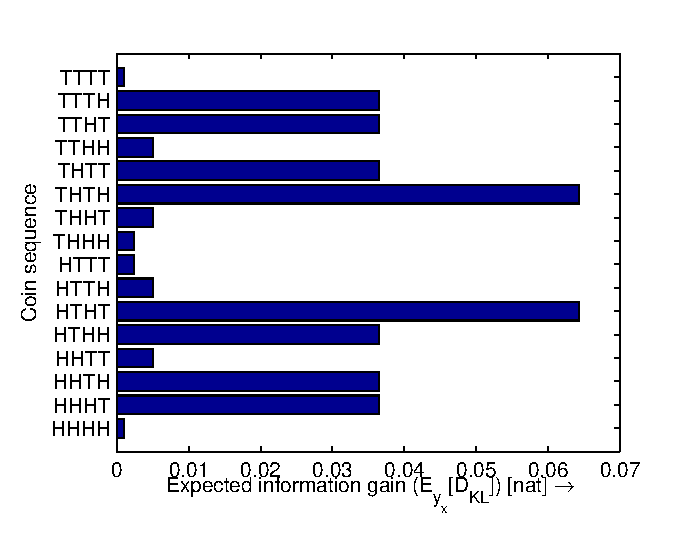
\includegraphics[width=3in]{img/coin.eps}
\caption{The information gain for all four flip coin sequences experiment prompts.}
\label{fig:coin}
\end{figure}

The most informative experiment prompts are the symmetric pair of coin sequences `HTHT' and `THTH'. To understand why: consider the models independently for the `HTHT' coin sequence. The bias coin observes two heads and two tails and infers that the bias should be centered around a fair weighting; this model does not favor either heads or tails as the next coin flip. In comparison, the Markov coin model infers that the flip sequence is alternating, and thus strongly favors the heads as the next coin flip in the sequence. By exploiting this difference in predictions, one can easily determine the underlying model from the response.

Following the same logic, the least informative experiment prompts are the symmetric pair of coin sequences `HHHH' and `TTTT'. Again, using the `HHHH' coin sequence as an example, the bias coin observes heads outcomes and thus infers that the coin is heavily biased towards heads outcome for the next coin. The Markov coin model infers that the flip sequence is unlikely to transition, and thus, also strongly favors a heads outcome for the next coin. Although each model has differing rationales for their predictions, they share the same prediction which makes it very difficult to determine the underlying model from an response.

Additionally, optimal experiment design can be used to gain general insights about both the experiment space and the candidate models. For example, the information gain is symmetric with respect to heads and tails symbol inversion. This should be expected as both models preserve their predictive distributions if the symbols are flipped. By observing general trends in the information gain of experiments, one can get a deeper understanding of the capabilities and limitations of the candidate models.

\subsection{Experiments?}

%    \begin{itemize}
%        \item Overview
%            \begin{itemize}
%                \item This case study is a toy example on disambiguating two models of subjective randomness
%                \item The purpose of this case study is to illustrate the pipeline of formalizing cognitive models using a probabilistic programming language and applying OED to find the optimal experiment
%            \end{itemize}
%        \item Models of subjective randomness
%            \begin{itemize}
%                \item We present two simple but plausible cognitive models of subjective randomness in the domain of random sequences
%                    \begin{enumerate}
%                        \item Independent flips from an identical coin
%                            \begin{itemize}
%                                \item Each event in the sequence is obtained from the same Bernoulli distribution
%                                \item The parameter of the Bernoulli distribution is inferred from the sequence
%                            \end{itemize}
%                        \item Flips from a Markov chain
%                            \begin{itemize}
%                                \item The sequence is generated from a Markov chain, where the outcome of an event depends on the previous event
%                                \item The transition parameter of the Markov chain is inferred from the sequence
%                            \end{itemize}
%                    \end{enumerate}
%                \item \emph{Include: graphical models of the two coin models}
%                \item \emph{Include: Church models of the two coin models}
%            \end{itemize}
%        \item Optimal experiment design
%            \begin{itemize}
%                \item We aim to present participants with a four event sequence and prompt them for the outcome of the next event
%                \item This is a simple experiment space with 16 possible prompts, which we exhaustively evaluate the information gain
%                \item \emph{Include: code example for invoking OED for this problem}
%            \end{itemize}
%        \item Results and discussion
%            \begin{itemize}
%                \item The optimal sequence is the symmetric pair of `0101' and '1010'
%                    \begin{itemize}
%                        \item The Markov model strongly predicts an alternating event, while the iid model does not favor either outcome
%                        \item The drastic difference between these predictions makes it easy to identify the underlying model
%                    \end{itemize}
%                \item The worst sequence is the symmetric pair of `0000' and '1111'
%                    \begin{itemize}
%                        \item Both models predict the same outcome, which is the repetition of the sequence
%                        \item As both models predict the same response, it is difficult to distinguish these models given this experiment prompt
%                    \end{itemize}
%                \item These results should agree with our intuitions about disambiguating these two models of subjective randomness
%                \item \emph{Include: plot of information gain for each sequence}
%            \end{itemize}
%    \end{itemize}

\section{Case study 2: Category learning}
\section{Relationship to previous work}
\section{Discussion}

The purpose of \red{our(?)} OED approach is to quantify the ability of an experiment to differentiate competing computational models. Our approach leverages Bayesian inference to reason about which model best describes a given phenomenon. By using the models' predictions to compute the likelihood of observing a particular response to an experiment, this approach provides a rational method for updating the change in belief about model uncertainty when such responses are observed. This change in belief is then quantified using information theoretic measures, and by maximizing these measures, OED allows one to find experiments that should maximally change the uncertainty of the beliefs in our models.

%\bibliographystyle{ieeetr}
%\bibliography{oed_nips_2016}

\end{document}
